\documentclass[14pt]{beamer}
\usepackage[T2A]{fontenc}
\usepackage[utf8]{inputenc}
\usepackage[english,russian]{babel}
\usepackage{amssymb,amsfonts,amsmath,mathtext}
\usepackage{cite,enumerate,float,indentfirst}
\usepackage[export]{adjustbox}
\usepackage{wrapfig}

\graphicspath{{images/}}

% The Beamer class comes with a number of default slide themes
% which change the colors and layouts of slides. Below this is a list
% of all the themes, uncomment each in turn to see what they look like.

%\usetheme{default}
%\usetheme{AnnArbor}
%\usetheme{Antibes}
%\usetheme{Bergen}
%\usetheme{Berkeley}
%\usetheme{Berlin}
%\usetheme{Boadilla}
\usetheme{CambridgeUS}
%\usetheme{Copenhagen}
%\usetheme{Darmstadt}
%\usetheme{Dresden}
%\usetheme{Frankfurt}
%\usetheme{Goettingen}
%\usetheme{Hannover}
%\usetheme{Ilmenau}
%\usetheme{JuanLesPins}
%\usetheme{Luebeck}
%\usetheme{Madrid}
%\usetheme{Malmoe}
%\usetheme{Marburg}
%\usetheme{Montpellier}
%\usetheme{PaloAlto}
%\usetheme{Pittsburgh}
%\usetheme{Rochester}
%\usetheme{Singapore}
%\usetheme{Szeged}
%\usetheme{Warsaw}

% As well as themes, the Beamer class has a number of color themes
% for any slide theme. Uncomment each of these in turn to see how it
% changes the colors of your current slide theme.

%\usecolortheme{albatross}
%\usecolortheme{beaver}
%\usecolortheme{beetle}
%\usecolortheme{crane}
%\usecolortheme{dolphin}
%\usecolortheme{dove}
%\usecolortheme{fly}
%\usecolortheme{lily}
%\usecolortheme{orchid}
%\usecolortheme{rose}
%\usecolortheme{seagull}
%\usecolortheme{seahorse}
%\usecolortheme{whale}
%\usecolortheme{wolverine}

%\setbeamertemplate{footline} % To remove the footer line in all slides uncomment this line
%\setbeamertemplate{footline}[page number] % To replace the footer line in all slides with a simple slide count uncomment this line

\setbeamertemplate{navigation symbols}{} % To remove the navigation symbols from the bottom of all slides uncomment this line

\setbeamercolor{footline}{fg=red}
\setbeamertemplate{footline}{
  \leavevmode%
  \hbox{%
  \begin{beamercolorbox}[wd=.333333\paperwidth,ht=2.25ex,dp=1ex,center]{}%
    М. И. Глухова (Мехмат ЮФУ)
  \end{beamercolorbox}%
  \begin{beamercolorbox}[wd=.333333\paperwidth,ht=2.25ex,dp=1ex,center]{}%
    Ростов-на-Дону, 2015
  \end{beamercolorbox}%
  \begin{beamercolorbox}[wd=.333333\paperwidth,ht=2.25ex,dp=1ex,right]{}%
  Стр. \insertframenumber{} из \inserttotalframenumber \hspace*{2ex}
  \end{beamercolorbox}}%
  \vskip0pt%
}

\newcommand{\itemi}{\item[\checkmark]}

\title{\small{Программная реализация алгоритмов поиска \\аналитических кривых на изображении}}
\vspace{15pt}%
\author{\small{%
М. И. Глухова\\%
\emph{Направление подготовки:}~Фундаментальная информатика и \\информационные технологии\\%
\emph{Руководитель:}~проф., д.ф.-м.н. В. С. Пилиди}\\%
\vspace{15pt}%
    Южный федеральный университет\\
	Институт математики, механики и компьютерных наук
    имени~И.\,И.\,Воровича%
}
\date{\small{Ростов-на-Дону, 2015}}

\begin{document}

%------------------------------------------------
\maketitle
%------------------------------------------------

\begin{frame}
\frametitle{Содержание} % Table of contents slide, comment this block out to remove it
\tableofcontents % Throughout your presentation, if you choose to use \section{} and \subsection{} commands, these will automatically be printed on this slide as an overview of your presentation
\end{frame}

%------------------------------------------------
\section{Постановка задачи}
%------------------------------------------------

\begin{frame}
\frametitle{Постановка задачи}
\begin{itemize}
  \item \textbf{Разработать алгоритм для поиска эллипсов на изображении.} 
  \item \textbf{Реализовать разработанный алгоритм.} 
  \item \textbf{Протестировать работу полученной программы.} 
\end{itemize}
\end{frame}

%------------------------------------------------
\section{Введение}
%------------------------------------------------

\begin{frame}
\frametitle{Введение}
\begin{figure}[H]
  \center
  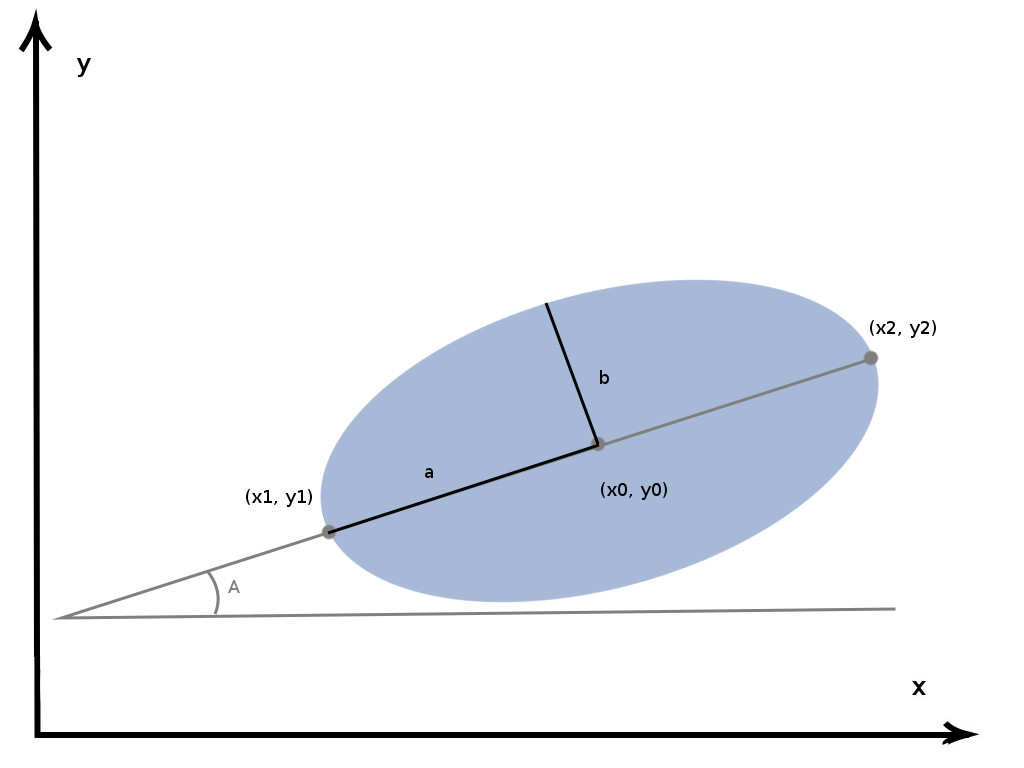
\includegraphics[width=0.6\linewidth]{ellipseparametres}
\end{figure}
\end{frame}

%------------------------------------------------
\begin{frame}
\frametitle{Параметры эллипса}
\begin{itemize}
  \item Каноническое уравнение
  $$ \frac{x^2}{a^2} + \frac{y^2}{b^2} = 1 $$
  \item Поворот
  $$ \frac{(x\cos \theta + y\sin A)^2}{a^2} + \frac{(x\sin A - y\cos A)^2}{b^2} = 1 $$
  \item Смещение
  \small
  $$ \frac{((x - x_0)\cos A + (y - y_0)\sin A)^2}{a^2}  + $$
  
  $$ \frac{((x - x_0)\sin A - (y - y_0)\cos A)^2}{b^2} = 1 $$
  \normalsize
\end{itemize}
\end{frame}
%------------------------------------------------

\section{Исследование предметной области}
\begin{frame}
\frametitle{Преобразование Хафа}
\begin{itemize}
  \item Определение параметров
  \item Голосование
  \item Выбор кандидатов   
\end{itemize}
\end{frame}

%------------------------------------------------

\begin{frame}
\frametitle{Основные применения}
\begin{itemize}
  \item Поиск прямых
  \item Поиск окружностей
  \item Поиск аналитических кривых
\end{itemize}
\end{frame}

%------------------------------------------------

\begin{frame}
\frametitle{Преобразование Хафа для аналитических кривых: подходы}
\begin{itemize}
  \item Рандомизация (Randomized Hough Transform)
  \item Вероятностный подход (Probabilistic Hough Transform)
  \item Поиск на уменьшенном изображении
\end{itemize}
\end{frame}

%------------------------------------------------
\section{Преобразование Хафа для поиска эллипсов}
%------------------------------------------------

%------------------------------------------------
\subsection{Одномерный аккумуляторный массив}
%------------------------------------------------
\begin{frame}
\frametitle{Одномерный аккумуляторный массив}
Алгоритм, предложенный в 2002 году, авторы: Yonghong Xie и Qiang Ji.
\begin{enumerate}
  \item Выбор двух краевых точек
  \item Определение центра, большой полуоси
  \item Определение малой полуоси голосованием
\end{enumerate}
\end{frame}

%------------------------------------------------
\begin{frame}
\frametitle{Оценки алгоритма}
\begin{itemize}
  \item Время: \(O(n^3)\), где \(n\) - количество ненулевых точек изображения
  \item Память: \(O(m)\), где \(m\) - размер изображения
\end{itemize}
\end{frame}

%------------------------------------------------
\subsection{Использование иерархической пирамиды}
%------------------------------------------------
\begin{frame}
\frametitle{Иерархическая пирамида}
\begin{figure}[H]
  \center
  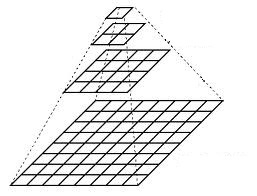
\includegraphics[width=0.6\linewidth]{Pyramid}
\end{figure}
\end{frame}

%------------------------------------------------
\begin{frame}
\frametitle{Алгоритм}
Алгоритм поиска эллипсов с использованием пирамидальной структуры данных изображения был предложен в 2011 году. Авторы: Chung-Fang Chien, Yu-Che Cheng, Ta-Te Lin.
\begin{enumerate}
  \item Построение иерархической пирамиды
  \item Поиск на изображении наименьшего размера
  \item Итеративное уточнение параметров
\end{enumerate}
\end{frame}

%------------------------------------------------
\section{Реализация}
%------------------------------------------------
\begin{frame}
\frametitle{Реализация}
\begin{itemize}
  \item Обе модификации объединены для большего ускорения
  \item Язык реализации: C++ (g++ версии 4.9.2)
  \item OpenCV 3.0
\end{itemize}
\end{frame}

%------------------------------------------------

\begin{frame}
\frametitle{Полученные результаты}
\begin{wrapfigure}{l}{0.32\linewidth} 
\vspace{-3ex}
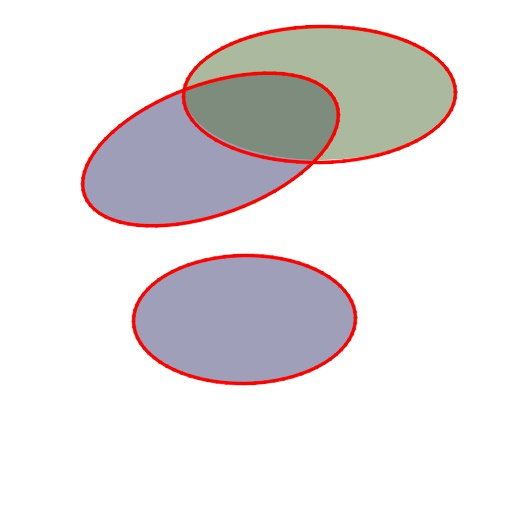
\includegraphics[width=0.32\textwidth,left]{res}
\label{fig:res}
\end{wrapfigure}
Найденные эллипсы:
\small
\begin{itemize}
  \item $(x_0 = 210, y_0 = 149, a = 133.795, b = 65, A = -0.343024)$
  \item $(x_0 = 319, y_0 = 94, a = 135.533, b = 68, A = -0.0221366)$
  \item $(x_0 = 244, y_0 = 319, a = 111.005, b = 64, A = -0.00900877)$
\end{itemize}
\normalsize
\end{frame}
%------------------------------------------------

\end{document} 
